\documentclass[oneside]{book}
\usepackage[utf8]{inputenc}
\usepackage{fancyhdr}
%\usepackage{listings}
\usepackage[document]{ragged2e}
\usepackage{lastpage}
\usepackage{circuitikz}
\usepackage{amsmath}
\usepackage{amssymb}
\usepackage{mathrsfs, amsmath}
\usepackage{amsfonts}
\usepackage{amsthm}
\usepackage{caption}
\usepackage{subcaption}
\usepackage{tcolorbox}
\usepackage{cancel}
\usepackage{nccmath}
\usepackage{wrapfig}
\usepackage{hyperref,lipsum}
\usepackage[export]{adjustbox}
%\usepackage{fullpage}
\usepackage{geometry}
\usepackage{listings}
\usepackage{textcomp}
\pagestyle{fancy}
\fancyhf{}
\fancyhead[L]{\leftmark} % Chapter name at the left header
\fancyhead[R]{\thepage} % Page number at the right header
\renewcommand{\chaptermark}[1]{\markboth{#1}{}}
\hypersetup{
    colorlinks=true,
    linkcolor=blue,
    filecolor=magenta,      
    urlcolor=cyan,
    pdftitle={Overleaf Example},
    pdfpagemode=FullScreen,
    }
\begin{document}
\begin{titlepage}
\centering
{\bfseries\Huge Indian Institute of Technology Hyderabad\par}


\vfill
\noindent
{\bfseries\Huge Elektronica Club  \par}
\bigskip%Título
\vspace{0.5cm}

{\bfseries\Large Signal Processing\par}
\vspace{0.5cm}
\noindent
\vfill
{\Large K Rahul\par}
{\Large ee23btech11027 \par}
\vfill
\end{titlepage}
\setcounter{page}{0}
\newpage
\tableofcontents
\newpage
\Large

\chapter{Introduction} \label{Chapter-1}
A PCB, or a Printed Circuit Board, is a board that can host a circuit template that can be used in many places. For example, the green board seen inside a home TV remote is a PCB, designed specifically for operating it. The base of the PCB is generally made up of a non-conductive material like fiberglass and the conductive pathway is generally made up of copper. The copper conductive layer helps in the interconnection between circuit components such as a resistor, capacitor, a microchip etc. \\ \bigskip

PCBs are generally mass manufactured as such an undertaking generally is less expensive. If the design of a particular electronic part has to be extremely compact, an IC is preferred, but if the size of the design is somewhat forgiving, a PCB can be used. As a sidenote, PCBs can also have ICs as their components, so PCBs can go hand-in-hand with ICs.

\newpage
\chapter{List out the characteristics of the system to be designed.}
The system to be designed is a DAC, a Digital to Analog Converter. All real world signals(be it sound, or the light intensities that make up a photograph) are analog signals. Systems that can operate directly on such analog signals are called analog systems, and these are generally pretty hard to make. Filtering in the analog domain for example, is much harder as compared to filtering in the digital domain. Hence, an analog signal has to first be converted to digital form that a computer can understand. This is taken care of by a system called the ADC(which in some sense is an "inverse" system of sorts for the DAC, which is what is going to be built).\\ \bigskip

After suitable analysis and manipulation, the digital form of the signal at times need to be converted back to analog form. For example, after carrying out filtering of analog signals on a computer, the filtered audio must be converted back to the analog domain for it to be heard as sound. This is taken care of by the DAC. A DAC takes in some number of bits(in our case, 3), and based on the value, figure out the output corresponding to those particular bits,

\newpage
\chapter{Working of the system and power rating}
The DAC is built using the following circuit.
\begin{figure}[htbp]
    \centering
    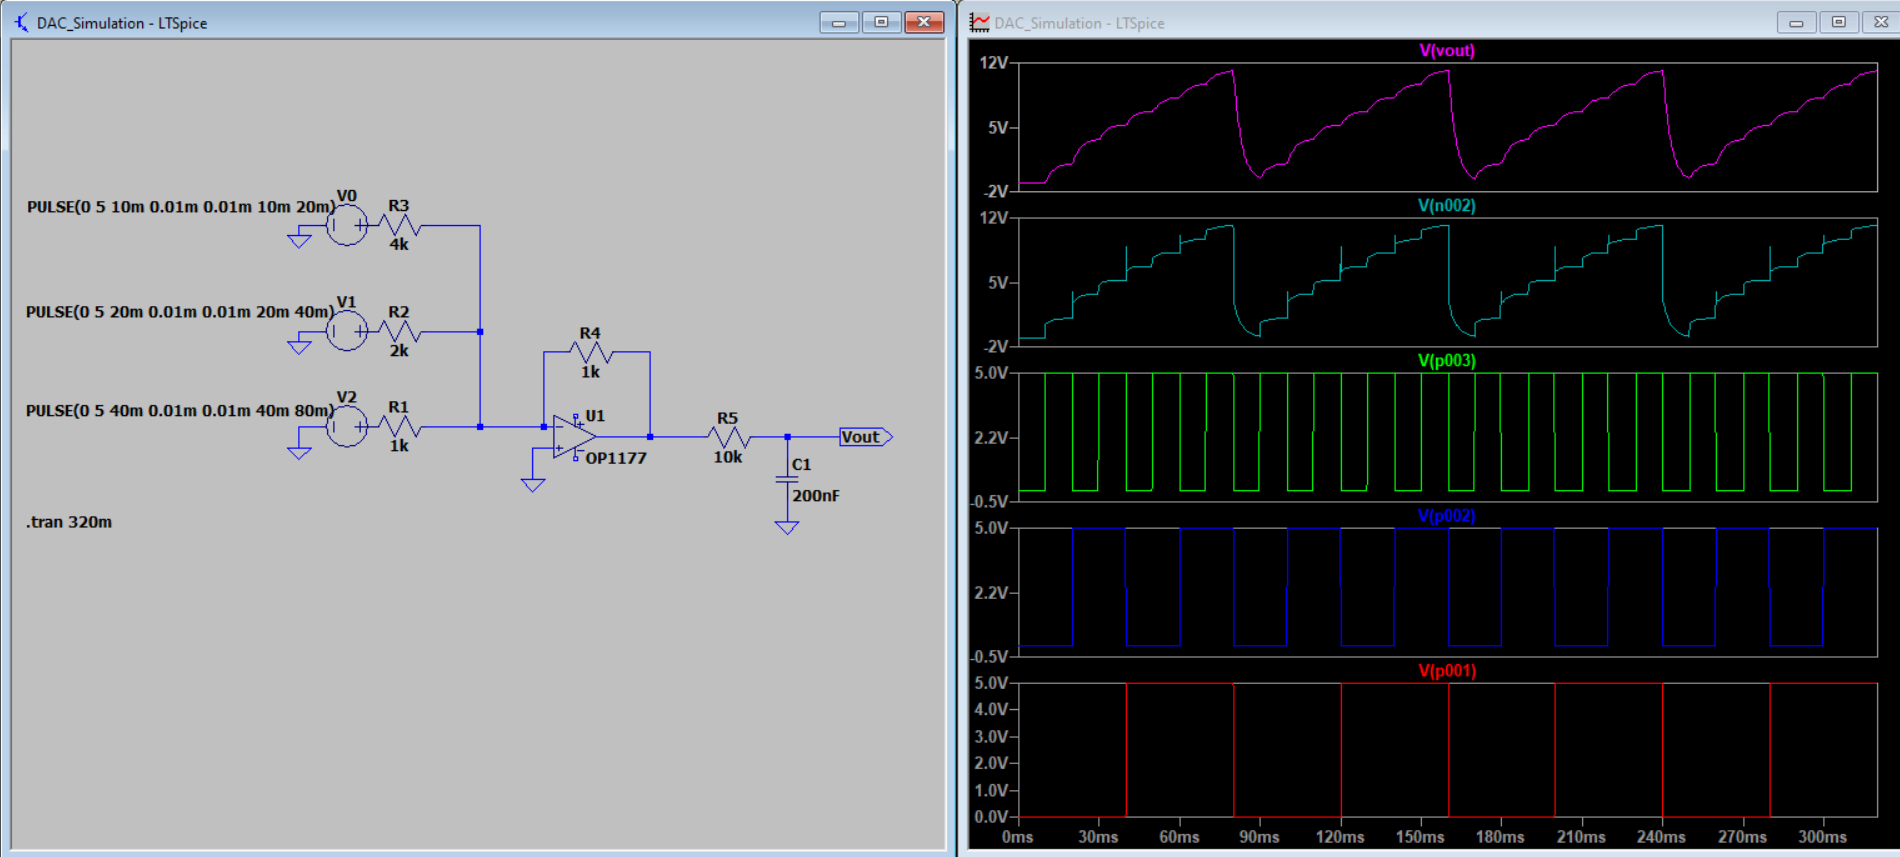
\includegraphics[width=1\textwidth]{figs/DAC Converter with Lowpass Filter - LTSpice.png}
    \caption{DAC Converter}
    \label{SPICE}
\end{figure} \\
\bigskip

In the oscilloscope readings(simulated ones from LTSpice\textsuperscript{\textregistered}),  the one marked V(p001) is $V_2$,  V(p002) is $V_1$, V(p003) is $V_0$, V(n002) is the output of the op-amp, and V(vout) is the output from the node labelled $V_{out}$.\\
Thing to note is that $V_0$, $V_1$, $V_2$\footnote{In the simulation above, each one of $V_0$, $V_1$ and $V_2$ is assumed to reach $5V$ in ON state and $0V $ in OFF state.} are the 3 bits, and the binary number is to be written as $V_2V_1V_0$, in that order. $V_0$ is the LSB and $V_2$ is the MSB. This DAC circuit\footnote{In particular, this circuit is known as a Binary Weighted DAC.} has been simulated in LTSpice\textsuperscript{\textregistered} as shown in the above figure.
Since a virtual ground exists at the junction(say, $P$) near the negative pin of the op-amp(the op-am can be safely considered to be an ideal one), and the op-amp takes in practically no current, a KCL equation can be set up at junction $P$.
\begin{align}
    V_{P} = -\biggl ( V_2 + \frac{V_1}{2} + \frac{V_0}{4} \biggr)
\end{align}
The value of $|V_P|$ has been noted for various values of $V_0$, $V_1$, $V_2$ as follows : 
\begin{table}[ht]
\centering
\setlength{\arrayrulewidth}{0.3mm}
\setlength{\tabcolsep}{15pt}
\renewcommand{\arraystretch}{1.5}



\begin{tabular}{ |p{2cm}|p{2cm}|p{2cm}|p{2cm}| }
\hline
$V_2$ & $V_1$ & $V_0$ & $V_P$\\
\hline
0 & 0 & 0 & 0\\
\hline
0 & 0 & 1 & 1.25 \\
\hline
0 & 1 & 0 & 2.5 \\
\hline
0 & 1 & 1 & 3.75 \\
\hline
1 & 0 & 0 & 5 \\
\hline
1 & 0 & 1 & 6.25 \\
\hline
1 & 1 & 0 & 7.5 \\
\hline
1 & 1 & 1 & 8.75 \\
\hline
\end{tabular}


\caption{Value of $V_P$}
\end{table} \\
\bigskip
As is evident, if $V_0$, $V_1$ and $V_2$ are taken to be the bits that make up a 3-bit number, the value of $V_P$ increases as the value of the bits themselves increase. \\
\bigskip
\newpage
As can be seen in the figure \autoref{SPICE}, in V(n002), the output of the op-amp, the signal is in the form of steps. This definitely is wrong, and can be reasoned easily. If a smooth wave is first passed through an ADC, it produces a stream of bits. Theoretically, if these stream of bits were to be put back into a DAC, they must produce back the same signal\footnote{notwithstanding the issue of number of bits, for now let us assume that the number of bits is sufficient to reconstruct the signal satisfactorily.}. But the output of the op-amp, however, is in the form of steps as remarked before. Hence, when a smooth wave is put into an ADC, and put into the above designed DAC, and output be generated from the output pin of the op-amp, we would not get back the same signal. \\ \bigskip
This entire detour is to draw attention to the fact that the output from the op-amp must be filtered using a lowpass filter in order to atleast approximately output the right signal. In our circuit, this has been carried out by a simple first-order RC lowpass filter, and the filtered output can be seen in V(vout), in figure \autoref{SPICE}  

\chapter{PCB Design}
The KiCAD EDA\textsuperscript{\textregistered} schematic and PCB layout for the aforementioned DAC can be found \href{https://github.com/HarryNyquist/Elektronica/tree/main/PCB/ADC_DAC_Converter/DAC_Converter%20-%20KiCAD}{\underline{\textbf{here}}}
\\ \bigskip
The LTSpice\textsuperscript{\textregistered} simulation for the same can be found \href{https://github.com/HarryNyquist/Elektronica/tree/main/PCB/ADC_DAC_Converter/DAC_Converter%20-%20LTSpice%20Simulations}{\underline{\textbf{here}}}
\end{document}
